\documentclass[fleqn, a4paper, 12pt, twoside]{article}
\usepackage{exsheets} %question and solution environments
\usepackage{amsmath, amssymb, amsthm} %standard AMS packages
\usepackage{esint} %integral signs
\usepackage{marginnote} %marginnotes
\usepackage{gensymb} %miscellaneous symbols
\usepackage{commath} %differential symbols
\usepackage{xcolor} %colours
\usepackage{cancel} %cancelling terms
\usepackage[free-standing-units]{siunitx} %formatting units
\usepackage{tikz, pgfplots} %diagrams
	\usetikzlibrary{calc, hobby, patterns, intersections, angles, quotes, spy}
\usepackage{graphicx} %inserting graphics
\usepackage{epstopdf} %converting and inserting eps graphics
\usepackage{hyperref} %hyperlinks
\usepackage{datetime} %date and time
\usepackage{ulem} %underline for \emph{}
\usepackage{xfrac, lmodern} %inline fractions
\usepackage{enumerate, enumitem} %numbered lists
\usepackage{float} %inserting floats
\usepackage[american voltages]{circuitikz} %circuit diagrams
\usepackage{pdflscape} %pages in landscape orientation
\usepackage{setspace} %double spacing
\usepackage{microtype} %micro-typography
\usepackage{listings} %formatting code
	\lstset{language=Matlab}
	\lstdefinestyle{standardMatlab}
	{
		belowcaptionskip=1\baselineskip,
		breaklines=true,
		frame=L,
		xleftmargin=\parindent,
		language=C,
		showstringspaces=false,
		basicstyle=\footnotesize\ttfamily,
		keywordstyle=\bfseries\color{green!40!black},
		commentstyle=\itshape\color{purple!40!black},
		identifierstyle=\color{blue},
		stringstyle=\color{orange},
	}
\usepackage{algpseudocode} %algorithms
\usepackage{algorithm} %algorithms
\usepackage{chronology}
\usepackage{qtree}
\usepackage{varwidth}
\usepackage{asymptote}

\newcommand\numberthis{\addtocounter{equation}{1}\tag{\theequation}} %adds numbers to specific equations in non-numbered list of equations

\theoremstyle{definition}
\newtheorem{example}{Example}
\newtheorem{definition}{Definition}

\theoremstyle{theorem}
\newtheorem{theorem}{Theorem}
\newtheorem{law}{Law}

\newcommand{\curl}{\mathrm{curl\,}}

\newcommand{\divergence}{\mathrm{div\,}}

\newcommand{\Arg}{\mathrm{Arg}}

\newcommand{\Int}{\mathrm{Int}}
\newcommand{\Ext}{\mathrm{Ext}}
\newcommand{\boundary}{\partial}

\makeatletter
\@addtoreset{section}{part} %resets section numbers in new part
\makeatother

\newcommand\blfootnote[1]{%
	\begingroup
	\renewcommand\thefootnote{}\footnote{#1}%
	\addtocounter{footnote}{-1}%
	\endgroup
}

\renewcommand{\marginfont}{\scriptsize \color{blue}}

\renewcommand{\tilde}{\widetilde}

\SetupExSheets{solution/print = true} %prints all solutions by default

%opening
\title{Complex Functions}
\author{Aakash Jog}
\date{2015-16}

\begin{document}

\maketitle
%\setlength{\mathindent}{0pt}

\blfootnote
{	
	\begin{figure}[H]
		
\includegraphics[height = 12pt]{cc.eps}
		\includegraphics[height = 12pt]{by.eps}
		\includegraphics[height = 12pt]{nc.eps}
		
\includegraphics[height = 12pt]{sa.eps}
	\end{figure}
	This work is licensed under the Creative Commons Attribution-NonCommercial-ShareAlike 4.0 International License. To view a copy of this license, visit \url{http://creativecommons.org/licenses/by-nc-sa/4.0/}.
} %CC-BY-NC-SA license

\tableofcontents

\newpage
\section{Lecturer Information}

\textbf{Zahi Hazan}\\
~\\
E-mail: \href{mailto:zahihaza@post.tau.ac.il}{zahihaza@post.tau.ac.il}\\

\section{Recommended Reading}

\begin{enumerate}
	\item James Ward Brown \& Ruel V. Churchill, ``Complex Variables and Applications'', McGraw-Hill, Inc. 1996.
	\item D. Zill, P. Shanahan, ``Complex Variables with Applications'', Jones and Bartlett Publishers.
\end{enumerate}

\section{Additional Reading}

\begin{enumerate}
	\item Saff, Edward B., and Arthur David Snider. Fundamentals of Complex Analysis with Applications to Engineering, Science, and Mathematics. 3rd ed. Upper Saddle River, NJ: Prentice Hall, 2002. ISBN: 0139078746.
	\item Sarason, Donald. Complex Function Theory. American Mathematical Society. ISBN: 0821886223
	\item Alfhors, Lars. Complex Analysis: An Introduction to the Theory of Analytic Functions of One Complex Variable. McGraw-Hill Education, 1979. ISBN: 0070006571.
\end{enumerate}

\newpage
\part{Complex Numbers}

\begin{definition}
	A number of the form
	\begin{align*}
		z & = x + i y
	\end{align*}
	where
	\begin{align*}
		i & = \sqrt{-1}    \\
		x & \in \mathbb{R} \\
		y & \in \mathbb{R}
	\end{align*}
	is called a complex number.
\end{definition}

\begin{definition}[Real part of a complex number]
	If
	\begin{align*}
		z & = x + i y
	\end{align*}
	then $x$ is called the real part of $z$, and is denoted as
	\begin{align*}
		x & = \Re(z)
	\end{align*}
\end{definition}

\begin{definition}[Imaginary part of a complex number]
	If
	\begin{align*}
		z & = x + i y
	\end{align*}
	then $y$ is called the imaginary part of $z$, and is denoted as
	\begin{align*}
		x & = \Im(z)
	\end{align*}
\end{definition}

\begin{definition}[Complex conjugate]
	If
	\begin{align*}
		z & = x + i y
	\end{align*}
	then
	\begin{align*}
		\overline{z} & = x - i y
	\end{align*}
	is called the complex conjugate of $z$.
\end{definition}

\begin{theorem}
	\begin{align*}
		z \overline{z} & = |z|^2
	\end{align*}
\end{theorem}

\begin{proof}
	\begin{align*}
		z                       & = x + i y \\
		\therefore \overline{z} & = x - i y
	\end{align*}
	Therefore,
	\begin{align*}
		z \overline{z} & = (x + i y) (x - i y)       \\
                               & = x^2 - i x y + i x y + y^2 \\
                               & = x^2 + y^2                 \\
                               & = |z|^2
	\end{align*}
\end{proof}

\begin{definition}[Polar representation]
	If
	\begin{align*}
		x & = r \cos \theta \\
		y & = r \sin \theta
	\end{align*}
	then $(r,\theta)$ is called the polar representation of $(x,y)$.
\end{definition}

\begin{theorem}[Euler's Formula]
	\begin{align*}
		r cos \theta + i r \sin \theta & = r e^{i \theta}
	\end{align*}
	\label{Euler's_Formula}
\end{theorem}

\begin{definition}[Absolute value or Norm]
	\begin{align*}
		|z| & = |x + i y| \\
                    & = \sqrt{x^2 + y^2}
	\end{align*}
	is called the absolute value, or the norm of $z$.
\end{definition}

\begin{theorem}
	\begin{equation*}
		|z| \le \left| \Re(z) \right| + \left| \Im(z) \right| \le \sqrt{2} |z|
	\end{equation*}
\end{theorem}

\begin{proof}
	\begin{gather*}
		\sqrt{x^2 + y^2} \le |x| + |y| \le \sqrt{2 x^2 + 2 y^2}\\
		\iff x^2 + y^2 \le x^2 + y^2 + 2 |x| |y| \le 2 x^2 + 2 y^2\\
		\iff x^2 + y^2 - 2 |x| |y| \ge 0\\
		\iff \left( |x| - |y| \right)^2 \ge 0
	\end{gather*}
\end{proof}

\begin{definition}[Argument]
	Let $z$ be a complex number.\\
Then, $\theta$, such that $\theta \in (-\pi,\pi]$, and
	\begin{align*}
		z & = (r,\theta)
	\end{align*}
	is called the argument of $z$.\\
	It is denoted as
	\begin{align*}
		\theta & = \Arg(z)
	\end{align*}
	If $\theta \notin (-\pi,\pi]$, but
	\begin{align*}
		z & = (r,\theta)
	\end{align*}
	then
	\begin{align*}
		\theta & = \arg(z)
	\end{align*}
\end{definition}

\begin{theorem}
	\begin{align*}
		z^n & = |z|^n e^{i n \Arg(z)}
	\end{align*}
\end{theorem}

\begin{proof}
	\begin{align*}
		z              & = |z| e^{i \Arg(z)}                                   \\
		\therefore z^n & = \left( |z| e^{i \Arg(z)} \right)^n                  \\
                               & = \left( |z| \right)^n \left( e^{i \Arg(z)} \right)^n \\
                               & = |z|^n e^{i n \Arg(x)}
	\end{align*}
\end{proof}

\begin{theorem}
	Let
	\begin{align*}
		z & = r e^{i \theta} \\
		w & = \rho e^{i \varphi}
	\end{align*}
	The solutions to
	\begin{align*}
		w & = \sqrt[n]{z}
	\end{align*}
	are
	\begin{align*}
		\varphi_k & = \frac{\theta}{n} + \frac{2 \pi k}{n}
	\end{align*}
	where $k \in \{0,\dots,n - 1\}$.
\end{theorem}

\begin{proof}
	\begin{align*}
		w              & = \sqrt[n]{z} \\
		\therefore w^n & = z
	\end{align*}
	Therefore,
	\begin{align*}
		\rho^n e^{i n \varphi} & = r e^{i \theta}
	\end{align*}
	Therefore, for $k \in \{0,\dots,n - 1\}$,
	\begin{align*}
		\rho               & = \sqrt[n]{r}      \\
		n \varphi          & = \theta + 2 \pi k \\
		\therefore \varphi & = \frac{\theta}{n} + \frac{2 \pi k}{n}
	\end{align*}
\end{proof}

\newpage
\part{Complex Sequences and Series}

\begin{definition}[Convergence of complex sequences]
	Let
	\begin{align*}
		z_n & = x_n + i y_n
	\end{align*}
	The sequence $\{z_n\}$ is said to converge to the limit $z = x + i y$, if $\forall \varepsilon > 0$, $\exists N$, such that $\forall n > N$, $|z_n - z| < \varepsilon$, i.e. there is a circular region of radius $\varepsilon$, centred at $z$, in which $z_n$ lies.
\end{definition}

\begin{theorem}
	$\{z_n\} \to z$, i.e. $\{z_n\}$ converges to $z$ if and only if all subsequences of $\{z_n\}$ converge to $z$.
\end{theorem}

\begin{question}
	Find the limit $\lim\limits_{n \to \infty} \frac{n + i}{2 n - i}$.
\end{question}

\begin{solution}
	\begin{align*}
		z_n & = \frac{n + i}{2 n - i}               \\
                    & = \frac{(n + i) (2 n + i)}{4 n^2 + 1} \\
                    & = \frac{2 n^2 + 1}{4 n^2 + 1} + i \frac{3 n}{4 n^2 + 1}
	\end{align*}
	Therefore,
	\begin{align*}
		\lim\limits_{n \to \infty} z_n & = \lim\limits_{n \to \infty} \frac{2 n^2 + 1}{4 n^2 + 1} + i \frac{3 n}{4 n^2 + 1} \\
                                               & = \frac{1}{2}
	\end{align*}
\end{solution}

\begin{question}
	Show that for
	\begin{align*}
		z_n & = -2 + \frac{(-1)^n}{n} i
	\end{align*}
	$\lim\limits_{n \to \infty} \Arg(z_n)$ does not exist, but $\lim\limits_{n \to \infty} |z_n|$ exists.
\end{question}

\begin{solution}
	The magnitude of $z_n$ is
	\begin{align*}
		|z_n| & = \left| -2 + \frac{(-1)^n}{n} i \right| \\
                      & = \sqrt{4 + \frac{(-1)^{2 n}}{n^2}}      \\
                      & = \sqrt{4 + \frac{1}{n^2}}
	\end{align*}
	Therefore,
	\begin{align*}
		\lim\limits_{n \to \infty} |z_n| & = \lim\limits_{n \to \infty} \sqrt{4 + \frac{1}{n^2}} \\
                                                 & = 2
	\end{align*}
	The argument of $z_{2 n}$ is
	\begin{align*}
		\Arg(z_{2 n})                                       & = \Arg\left( -2 + \frac{(-1)^{2 n}}{2 n} i \right)                 \\
		\therefore \lim\limits_{n \to \infty} \Arg(z_{2 n}) & = \lim\limits_{n \to \infty} \Arg\left( -2 + \frac{i}{2 n} \right) \\
                                                                    & = \pi
	\end{align*}
	The argument of $z_{2 n + 1}$ is
	\begin{align*}
		\Arg(z_{2 n + 1})                                   & = \Arg\left( -2 + \frac{(-1)^{2 n + 1}}{2 n + 1} i \right)         \\
		\therefore \lim\limits_{n \to \infty} \Arg(z_{2 n}) & = \lim\limits_{n \to \infty} \Arg\left( -2 - \frac{i}{2 n} \right) \\
                                                                    & = -\pi
	\end{align*}
	Therefore, as the limit of two subsequences are not equal, the limit does not exist.
\end{solution}<++>

\newpage
\part{Topology on the Complex Plane}

\begin{definition}[Neighbourhood of a complex number]
	A circular region of radius $\varepsilon$ centred at $z$, is called the $\varepsilon$ neighbourhood of $z$.
	\begin{equation*}
		B(z,\varepsilon) = D(z,\varepsilon) = \left\{ w \in \mathbb{C} : |w - z| < \varepsilon \right\}
	\end{equation*}
	\begin{figure}[h]
		\centering
		\begin{tikzpicture}
			\def\xMIN{-1};
			\def\xMAX{4};
			\def\yMIN{-1};
			\def\yMAX{4};
	
			\coordinate (z) at (2,2);
	
			\def\epsilon{0.8};
	
			\begin{scope}[stealth-stealth]
				\draw (\xMIN,0) -- (\xMAX,0) node [right] {$\Re$};
				\draw (0,\yMIN) -- (0,\yMAX) node [above] {$\Im$};
			\end{scope}
	
			\begin{scope}
				\draw [fill = lightgray] (z) circle (\epsilon);
	
				\draw [-stealth] (z) -- ++(30:\epsilon) node [midway, below] {$\varepsilon$};
			\end{scope}

			\begin{scope}
				\filldraw (z) circle (1pt) node [below] {$z$};
			\end{scope}
		\end{tikzpicture}
		\caption{Neighbourhood of a complex number}
	\end{figure}
\end{definition}

\begin{definition}[Interior point]
	Let $A \subseteq \mathbb{C}$.\\
	$z \in \mathbb{C}$ is called an inner or interior point of $A$ if there exists at least one $\varepsilon_z > 0$, such that $B(z,\varepsilon_z) \subset A$.\\
	The set of all interior points of $A$ is denoted by $\Int(A)$ or $A^{\circ}$.
\end{definition}

\begin{definition}[Exterior point]
	Let $A \subseteq \mathbb{C}$.\\
	$z \in \mathbb{C}$ is called an outer or exterior point of $A$ if there exists at least one $\varepsilon_z > 0$, such that $B(z,\varepsilon_z) \subset (\mathbb{C} \setminus A)$.
	The set of all exterior points of $A$ is denoted by $\Ext(A)$.
\end{definition}

\begin{definition}[Edge point]
	Let $A \subseteq \mathbb{C}$.\\
	$z \in \mathbb{C}$ is called an edge or boundary point of $A$ if it is neither an inner point of $A$, nor an outer point of $A$.
	The set of all boundary points of $A$ is denoted by $\boundary(A)$.
\end{definition}

\begin{definition}[Open set]
	A set $A \subseteq \mathbb{C}$ is called an open set if $A = A^{\circ}$, i.e. for any point $z \in A$, $\exists \varepsilon > 0$, such that $D(z,\varepsilon) \subset A$.
\end{definition}

\begin{definition}[Closer of a set]
	The closer of $A$ is defined to be
	\begin{align*}
		\overline{A} &= A^{\circ} \cup \boundary A
	\end{align*}
\end{definition}

\begin{definition}[Closed set]
	A set $A$ is called a closed set if $\boundary A \subset A$, i.e. $A = \overline{A}$.
\end{definition}

\begin{definition}[Connected set]
	A set $A$ is called a connected set of for any $z_1,z_n \in A$, there exists a polygonal path, i.e. a finite set of connected straight lines, which connects $z_1$ and $z_2$, and belongs to $A$.
\end{definition}

\begin{definition}[Domain]
	An open connected set is called a domain.
\end{definition}

\begin{definition}[Bound set]
	A set $A$ is said to be a bound set if it is bound inside a disk.
\end{definition}

\begin{question}
	Describe geometrically and list the properties of the following sets.
	\begin{enumerate}
		\item $A = \left\{ z \in \mathbb{C} : \Re(z) \ge 2 , \Im(z) \le 4 \right\}$
		\item $B = \left\{ z \in \mathbb{C} : |z - 1 + 3 i| > 3 \right\}$
	\end{enumerate}
\end{question}

\begin{solution}
	\begin{enumerate}[leftmargin=*]
		\item
			$A$ is the union of the bottom half plane with respect to the line $y = 4$, and the right half plane with respect to the line $x = 2$.
			\begin{figure}[H]
				\centering
				\begin{tikzpicture}[scale = 0.7]
					\def\xMIN{-6};
					\def\xMAX{6};
					\def\yMIN{-6};
					\def\yMAX{6};

					\begin{scope}
						\draw (\xMIN,0) -- (\xMAX,0) node [right] {$\Re$};
						\draw (0,\yMIN) -- (0,\yMAX) node [above] {$\Im$};
					\end{scope}

					\begin{scope}
						\fill [red, opacity = 0.5] (2,4) rectangle (\xMAX,\yMIN);
					\end{scope}

					\begin{scope}[stealth-stealth]
						\draw (\xMIN,0) -- (\xMAX,0);
						\draw (0,\yMIN) -- (0,\yMAX);
					\end{scope}
				\end{tikzpicture}
			\end{figure}
			Therefore, as $A = A^{\circ} + \boundary A$, it is a closer, unbounded set.
		\item
			$A$ is the complement of a disk, centred at $1 - 3 i$, with radius $3$.
			\begin{figure}[H]
				\centering
				\begin{tikzpicture}[scale = 0.7]
					\def\xMIN{-8};
					\def\xMAX{8};
					\def\yMIN{-8};
					\def\yMAX{8};

					\begin{scope}
						\draw (1,-3) circle (1pt) node [above left] {$1 - 3 i$};
					\end{scope}

					\begin{scope}
						\fill [red, opacity = 0.5] (\xMIN,\yMIN) rectangle (\xMAX,\yMAX);
						\fill [white] (1,-3) circle (3);
					\end{scope}

					\begin{scope}[stealth-stealth]
						\draw (\xMIN,0) -- (\xMAX,0) node [right] {$\Re$};
						\draw (0,\yMIN) -- (0,\yMAX) node [above] {$\Im$};
					\end{scope}
				\end{tikzpicture}
			\end{figure}
			Therefore, it is an open, unbounded set.
	\end{enumerate}
\end{solution}

\begin{question}
	Prove that the upper half plane $U = \left\{ z : \Im(z) > 0 \right\}$ is open.
\end{question}

\begin{solution}
	Let
	\begin{align*}
		z & = x + i y
	\end{align*}
	Therefore, as $z \in U$, $y > 0$.\\
	Therefore, consider the disk $D\left( z , \frac{y}{2} \right)$.\\
	Let $w \in D\left( z , \frac{y}{2} \right)$.
	Therefore,
	\begin{align*}
		|w - z|                              & < \frac{y}{2} \\
		\therefore \left| \Im(w - z) \right| & \le |w - z|   \\
                                                     & \le \frac{y}{2}
	\end{align*}
	Therefore,
	\begin{gather*}
		-\frac{y}{2} \le \Im(w) - \Im(z) \le \frac{y}{2}\\
		\therefore -\frac{y}{2} \le \Im(w) - y \le \frac{y}{2}\\
		\therefore \Im(w) \ge \frac{y}{2} > 0
	\end{gather*}
	Therefore, as $\Im(w) > 0$, $w \in U$.
	Therefore, $U$ is open.
	\qed
\end{solution}

\newpage
\part{Complex Functions}

\section{Complex Functions}

\begin{definition}[Complex function]
	Let $A \subseteq \mathbb{C}$.
	$f : A \to \mathbb{C}$ is called a complex function, which matches $z \in A$ to $f(z) \in \mathbb{C}$.
\end{definition}

\begin{theorem}
	Any complex function $f$ can be written as
	\begin{align*}
		f(x + i y) & = \Re f(x + i y) + i \Im f(x + i y) \\
                           & = u(x,y) + i v(x,y)
	\end{align*}
\end{theorem}

\section{Limits}

\begin{definition}
	Let $f$ be a complex function defined on a neighbourhood of $z_0$, but may or may not be defined at $z_0$.
	Then, the limit of $f(z)$ at $z_0$ is defined as
	\begin{align*}
		w & = \lim\limits_{z \to z_0} f(z)
	\end{align*}
	if $\forall \varepsilon > 0$, $\exists \delta > 0$, such that $\forall z \in \mathbb{X}$such that $|z - z_0| < \delta$, $\left| f(z) - w \right| < \varepsilon$.
\end{definition}

\begin{question}
	Show that
	\begin{align*}
		\lim\limits_{z \to 1} \frac{i z}{2} & = \frac{i}{2}
	\end{align*}
\end{question}

\begin{solution}
	Let $|z - 1| < \delta$.
	Therefore, for $\varepsilon > 0$,
	\begin{align*}
		\left| f(z) - \frac{i}{2} \right| & = \left| \frac{i z}{2} - \frac{i}{2} \right| \\
                                                  & = \left| \frac{i}{2} \right| |z - 1|         \\
                                                  & = \frac{1}{2} \left| z - i \right|
	\end{align*}
	Therefore, for $\delta \le 2 \varepsilon$, $\left| f(z) - \frac{i}{2} \right| < \varepsilon$.
	\qed
\end{solution}

\end{document}
